\documentclass[12pt]{article}

% CSCE 763 template style adapted for EMCH homework
\usepackage{amsmath}
\usepackage{amssymb}
\usepackage{amsfonts}
\usepackage{graphicx}
\usepackage{tikz}
\usepackage{pgfplots}
\usepackage[margin=1in]{geometry}
\usepackage{xcolor}
\usepackage{enumitem}
\usepackage{tcolorbox}
\usepackage{fancyhdr}
\usepackage{booktabs}
\usepackage{array}
\usepackage{colortbl}
\usepackage{float}
\usepackage{tabularx}
\usepackage{multicol}
\usepackage{listings}

\pgfplotsset{compat=1.17}
\usetikzlibrary{shapes.geometric, arrows.meta, positioning, patterns}

% --- USC Brand Colors (from CSCE 763 template) ---
\definecolor{USC_Garnet}{HTML}{73000A}
\definecolor{USC_Sandstorm}{HTML}{FFF2E3}
\definecolor{USC_Black90}{HTML}{363636}
\definecolor{USC_Black70}{HTML}{5C5C5C}
\definecolor{USC_Black50}{HTML}{A2A2A2}
\definecolor{USC_Black10}{HTML}{ECECEC}
\definecolor{USC_Honeycomb}{HTML}{65780B}
\definecolor{USC_Atlantic}{HTML}{466A9F}
\definecolor{USC_Congaree}{HTML}{1F414D}
\definecolor{USC_Rose}{HTML}{CC2E40}

\pagestyle{fancy}
\setlength{\headheight}{14.5pt}
\fancyhf{}
\fancyhead[L]{Page \thepage}
\fancyhead[C]{CSCE 763}
\fancyhead[R]{JC Vaught}
\renewcommand{\headrulewidth}{0pt}

\newtcolorbox{stepbox}[1][Step]{
  colback=white,
  colframe=USC_Garnet,
  fonttitle=\bfseries,
  title=#1,
  sharp corners,
  colbacktitle=USC_Garnet,
  coltitle=white,
}

\newtcolorbox{resultsbox}{
  colback=white,
  colframe=USC_Honeycomb,
  fonttitle=\bfseries,
  title=Results,
  sharp corners,
  colbacktitle=USC_Honeycomb,
  coltitle=white,
}

\newcommand{\question}[1]{%
  \clearpage
  \vspace{0.5cm}
  {\noindent\normalsize \textbf{#1}}
  \vspace{0.2cm}
  \hrule
  \vspace{0.1cm}
  \hrule
  \vspace{0.3cm}
}

\newcommand{\questionpart}[1]{%
  \clearpage
  \vspace{0.5cm}
  {\noindent\normalsize \textbf{#1}}
  \vspace{0.2cm}
  \hrule
  \vspace{0.1cm}
  \hrule
  \vspace{0.3cm}
}

\setlist[enumerate,1]{label=\arabic*.}
\setlist[enumerate,2]{label=(\alph*)}

\lstset{language=Matlab,
        basicstyle=\ttfamily\small,
        keywordstyle=\color{blue},
        commentstyle=\color{gray},
        stringstyle=\color{red},
        breaklines=true,
        frame=single,
        showstringspaces=false,
        numbers=left,
        numberstyle=\tiny\color{gray},
        stepnumber=1}

\graphicspath{{./}{figures/}}
\title{EMCH 367 Controls \\ Homework \#4}
\author{Jacob C. Vaught}
\date{Fall 2024}

\begin{document}
\maketitle
\setlength{\parindent}{0pt}

\begin{center}
\begin{tcolorbox}[colback=white, colframe=gray!50!black, colbacktitle=gray!20!white,
                  coltitle=black, sharp corners, boxrule=1pt,
                  title=\Large\bfseries Table of Contents]
\begin{tabular}{p{0.82\textwidth}r}
\textbf{Problem 1 (50pt)} \dotfill & \textbf{\pageref{quest:1}} \\[0.3em]
\textbf{Problem 2 (30pt)} \dotfill & \textbf{\pageref{quest:2}} \\[0.3em]
\textbf{Problem 3 (20pt)} \dotfill & \textbf{\pageref{quest:3}} \\[0.3em]
\textbf{Bonus Problem (20pt)} \dotfill & \textbf{\pageref{quest:4}} \\n\end{tabular}
\vspace{0.2cm}
\end{tcolorbox}
\end{center}


\question{Problem 1 (50 pt)}\label{quest:1}
\begin{stepbox}[Step 1: Approach]
Work through each requested subpart and show supporting derivations.
\end{stepbox}

Consider the closed-loop transfer function given by:
\[
G_{cl}(s) = \frac{25(s + 2)}{(s + 1)(s + 5)(s + 10)}.
\]

\begin{enumerate}
    \item[(a)] (20 pt) \textbf{Standard Form and Bode Diagram}

    \textbf{Standard Form:}  
    In control systems, expressing a transfer function in \textit{standard form} involves rewriting each term of the transfer function such that it is represented as \(\frac{s}{\omega_0} + 1\), where \(\omega_0\) is the corner (or break) frequency. This form is particularly useful for constructing Bode diagrams, as it simplifies the analysis of the system's frequency response by standardizing the representation of poles and zeros.

    \textbf{Rewriting \( G_{cl}(s) \) in Standard Form:}  
    To express \( G_{cl}(s) \) in standard form, we factor out the coefficients of \( s \) in each term:

    \[
    G_{cl}(s) = \frac{25(s + 2)}{(s + 1)(s + 5)(s + 10)} = \frac{25\left(\frac{s}{2} + 1\right)}{\left(\frac{s}{1} + 1\right)\left(\frac{s}{5} + 1\right)\left(\frac{s}{10} + 1\right)}.
    \]

    Here, each term is now in the form \(\frac{s}{\omega_0} + 1\), where:
    \begin{align*}
        \omega_0 \text{ (numerator zero)} &= 2 \text{ rad/s}, \\
        \omega_1 \text{ (first denominator pole)} &= 1 \text{ rad/s}, \\
        \omega_2 \text{ (second denominator pole)} &= 5 \text{ rad/s}, \\
        \omega_3 \text{ (third denominator pole)} &= 10 \text{ rad/s}.
    \end{align*}

    \textbf{Final Transfer Function in Standard Form:}
    \[
    G_{cl}(s) = \frac{25\left(\frac{s}{50} + 1\right)}{\left(\frac{s}{1} + 1\right)\left(\frac{s}{5} + 1\right)\left(\frac{s}{10} + 1\right)}.
    \]
    
\newpage
\subsection*{Bode Diagrams}

The Bode diagrams for \( G_{cl}(s) \) over the frequency range \( \omega = 0.01 \) rad/s to \( \omega = 100 \) rad/s are shown below.

\begin{figure}[h!]
    \centering
    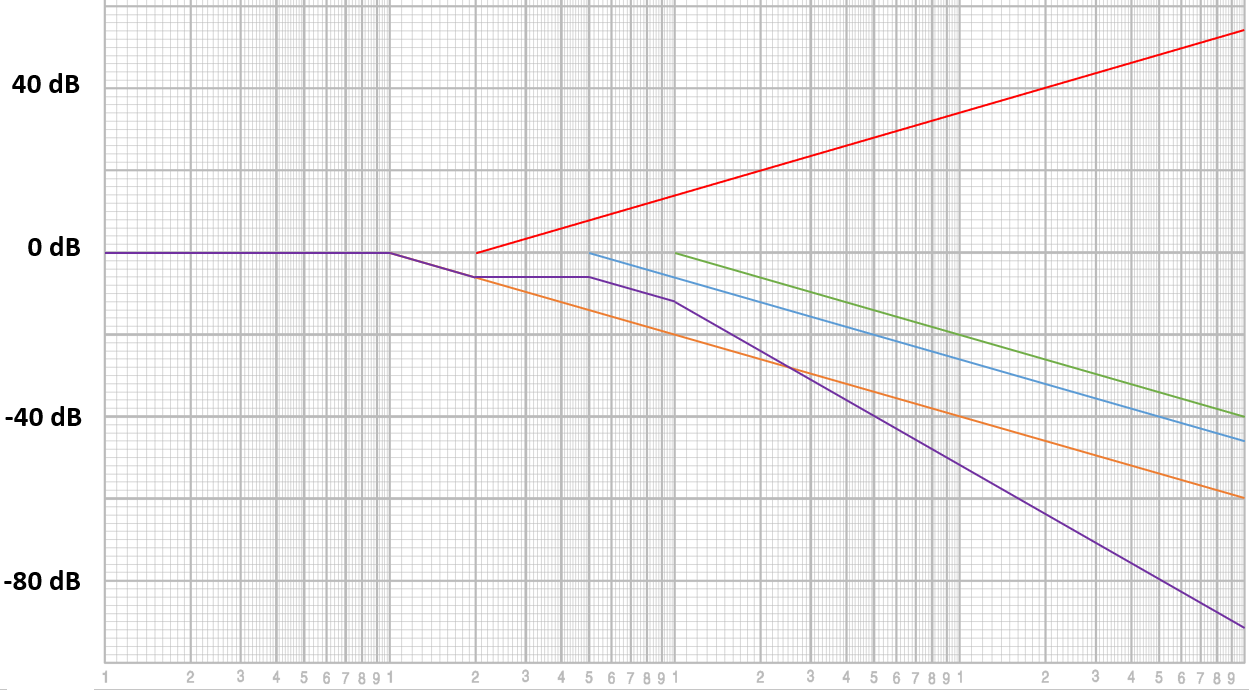
\includegraphics[width=0.8\textwidth]{magnitude.png}
    \caption{Bode Magnitude Plot}
    \label{fig:bode_magnitude_matlab}
\end{figure}

\begin{figure}[h!]
    \centering
    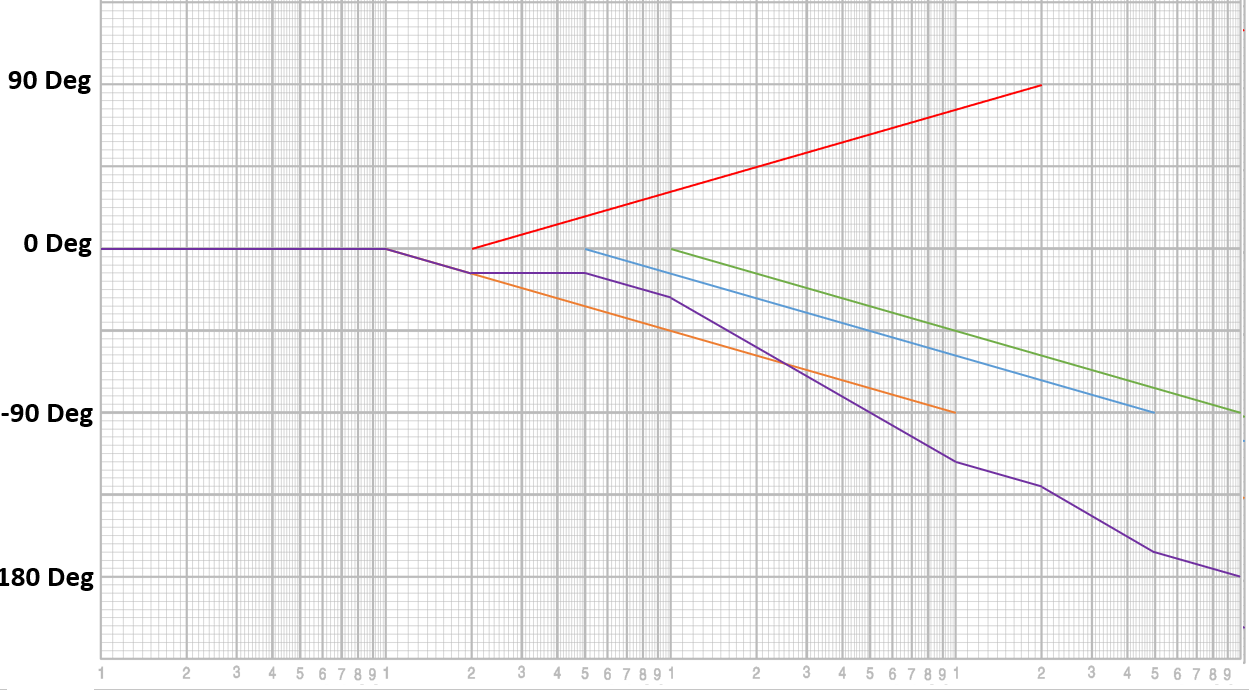
\includegraphics[width=0.8\textwidth]{phase.png}
    \caption{Bode Phase Plot}
    \label{fig:phase}
\end{figure}

\newpage
    \item[(b)] (10 pt) Draw the Bode diagram of $G_{cl}(s)$ using MATLAB.

\begin{lstlisting}[caption={BodePlot\_Gcl.m}]
% BodePlot_Gcl.m
% MATLAB code to plot Bode diagram of G_cl(s) = 25(s + 2)/[(s + 1)(s + 5)(s + 10)]

% Define numerator and denominator
numerator = 25 * [1 2]; % 25(s + 2)
denominator = conv(conv([1 1], [1 5]), [1 10]); % (s + 1)(s + 5)(s + 10)

% Create transfer function
Gcl = tf(numerator, denominator);

% Plot Bode diagram
bode(Gcl)
grid on
title('Bode Diagram of G_{cl}(s)')
\end{lstlisting}

\begin{figure}[h!]
    \centering
    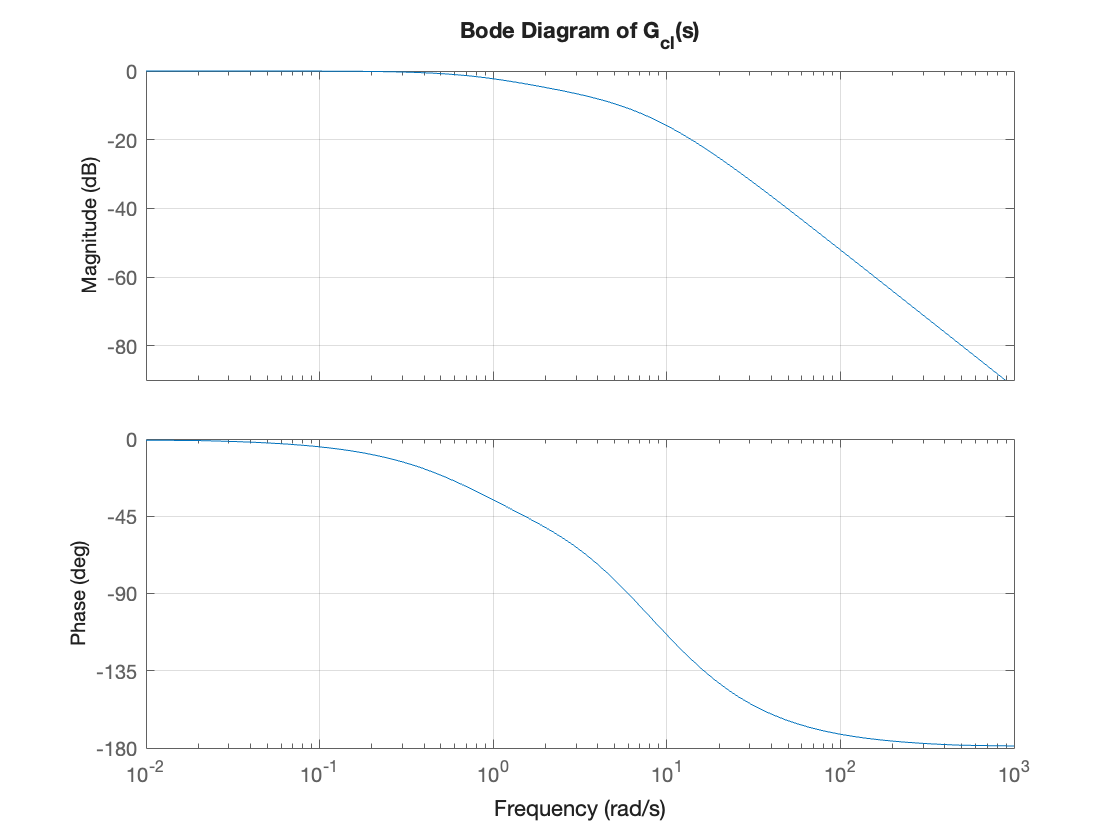
\includegraphics[width=0.95\textwidth]{bode.png}
    \caption{Bode Magnitude Plot from MATLAB}
    \label{fig:nyquist_open_loop}
\end{figure}

\newpage
    \item[(c)] (10 pt) Draw the Nyquist plot using MATLAB. \textit{(Hint: First, find the open-loop transfer function.)}
\begin{lstlisting}[caption={NyquistPlot\_Gcl.m}]
% NyquistPlot_Gcl.m
% MATLAB code to plot Nyquist plot of the open-loop transfer function G(s)

% Define numerator and denominator of G_cl(s)
numerator_cl = 25 * [1 2]; % 25(s + 2)
denominator_cl = conv(conv([1 1], [1 5]), [1 10]); % (s + 1)(s + 5)(s + 10)

% Create closed-loop transfer function
Gcl = tf(numerator_cl, denominator_cl);

% Calculate open-loop transfer function G(s) = Gcl / (1 - Gcl)
G = Gcl / (1 - Gcl);

% Plot Nyquist plot
nyquist(G)
grid on
title('Nyquist Plot of Open-Loop Transfer Function G(s)')
\end{lstlisting}
\begin{figure}[h!]
    \centering
    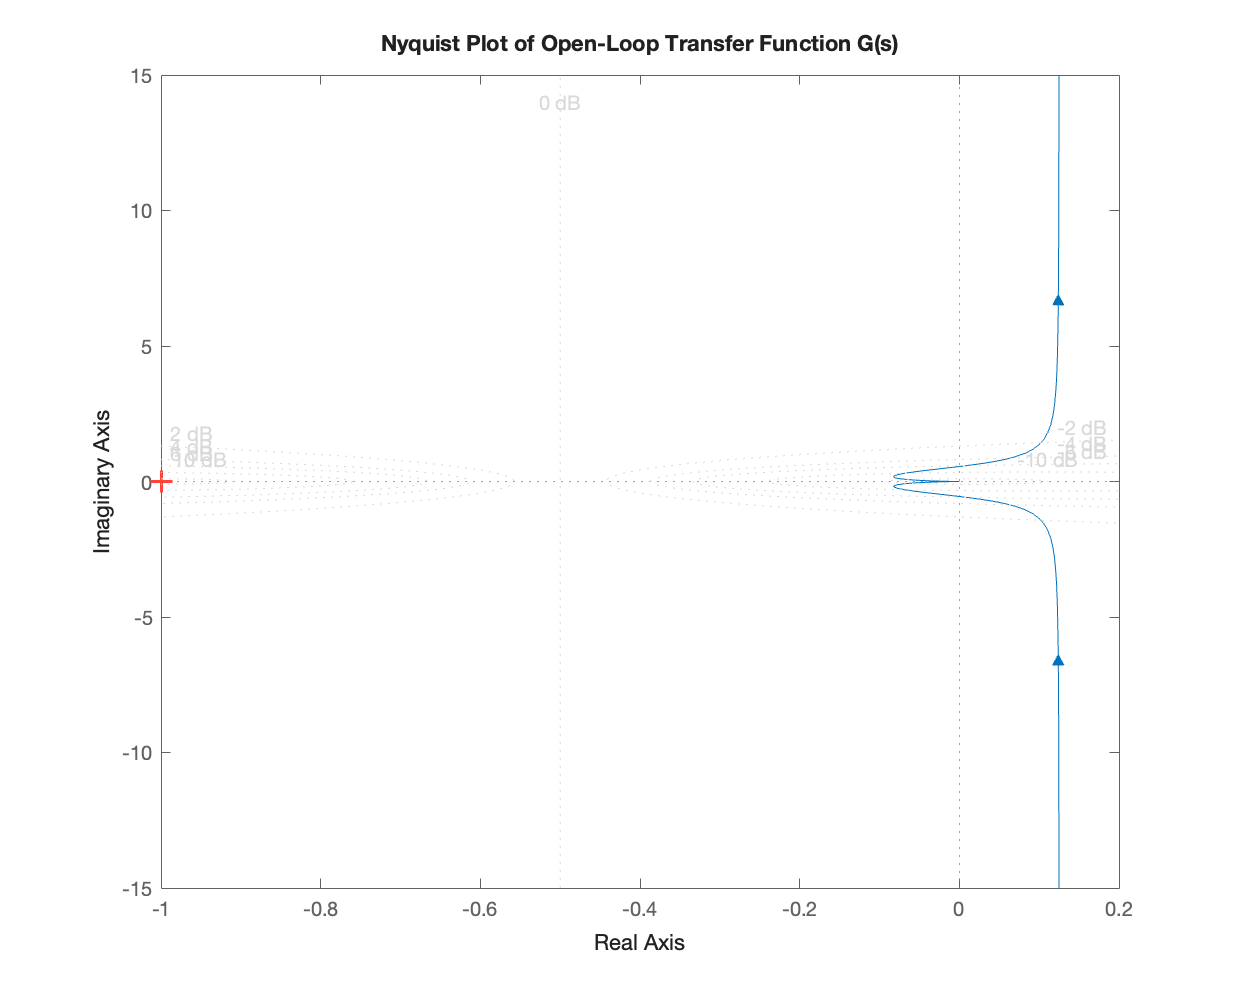
\includegraphics[width=0.9\textwidth]{nyquist.png}
    \caption{Nyquist Plot from MATLAB}
    \label{fig:nyquist_p2a}
\end{figure}

    \item[(d)] (10 pt) Analyze the stability of the closed-loop system using the Nyquist stability criterion.

    System is \textbf{stable} since the Nyquist plot does not cross the critical point.
\end{enumerate}

\begin{resultsbox}
Final answers for the previous problem are summarized in the work above.
\end{resultsbox}

\question{Problem 2 (30 pt)}\label{quest:2}
\begin{stepbox}[Step 1: Approach]
Work through each requested subpart and show supporting derivations.
\end{stepbox}

\begin{enumerate}
    \item[(a)] (15 pt) \textbf{Nyquist Plot and Stability Analysis}

    \textbf{Problem Statement:}  
    Consider a unity feedback control system with the following open-loop transfer function:
    \[
    G(s) = \frac{s^2 + 2s + 1}{s^3 + 0.2s^2 + s + 1}.
    \]
    \begin{enumerate}
        \item \textbf{Nyquist Plot:}  
        Draw the Nyquist plot of \( G(s) \) using MATLAB over a suitable range of frequencies.
        
        \item \textbf{Stability Examination:}  
        Analyze the Nyquist plot to determine the stability of the closed-loop system. Apply the Nyquist Stability Criterion to assess whether the system is stable. \textbf{UNSTABLE}
    \end{enumerate}


    \textbf{MATLAB Code:}
    \begin{verbatim}
    % Define the numerator and denominator of G(s)
    num = [1 2 1];
    den = [1 0.2 1 1];
    
    % Create the transfer function
    G = tf(num, den);
    
    % Plot the Nyquist diagram
    nyquist(G);
    grid on;
    title('Nyquist Plot of G(s) = (s^2 + 2s + 1)/(s^3 + 0.2s^2 + s + 1)');
    \end{verbatim}
    \begin{figure}[h!]
    \centering
    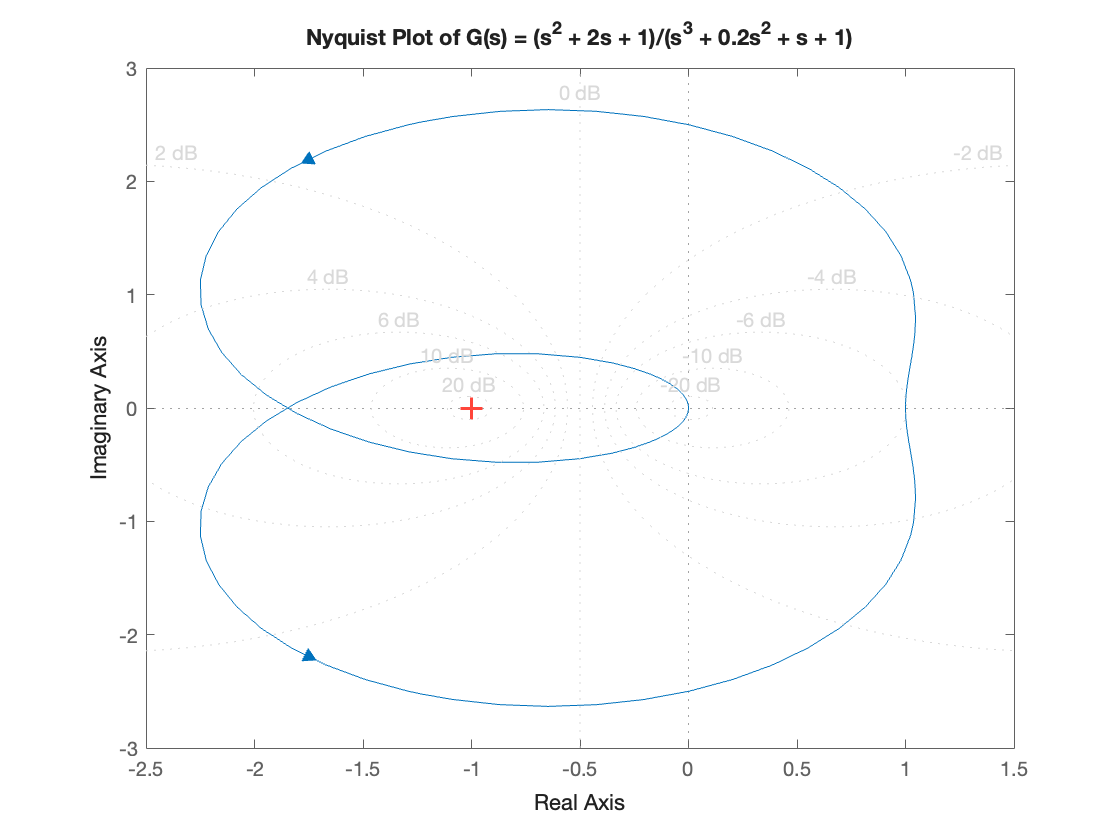
\includegraphics[width=0.9\textwidth]{p2a.png}
    \caption{Nyquist Plot from MATLAB}
    \label{fig:nyquist_p2b}
\end{figure}

    \item[(b)] (15 pt) \textbf{Nyquist Plot and Stability Analysis}

    \textbf{Problem Statement:}  
    Consider a unity feedback control system with the following open-loop transfer function:
    \[
    G(s) = \frac{100(s + 1)}{s(s + 5)(s^2 + 2s + 5)}.
    \]
    \begin{enumerate}
        \item \textbf{Nyquist Plot:}  
        Draw the Nyquist plot of \( G(s) \) using MATLAB over a suitable range of frequencies.
        
        \item \textbf{Stability Examination:}  
        Analyze the Nyquist plot to determine the stability of the closed-loop system. Apply the Nyquist Stability Criterion to assess whether the system is stable. \textbf{UNSTABLE}
    \end{enumerate}

   
    \textbf{MATLAB Code:}
    \begin{verbatim}
    % Define the numerator and denominator of G(s)
    num = [100 100];
    den = conv([1 0], conv([1 5], [1 2 5]));
    
    % Create the transfer function
    G = tf(num, den);
    
    % Plot the Nyquist diagram
    nyquist(G);
    grid on;
    title('Nyquist Plot of G(s) = 100(s + 1)/(s(s + 5)(s^2 + 2s + 5))');
    \end{verbatim}
\end{enumerate}
    \begin{figure}[h!]
    \centering
    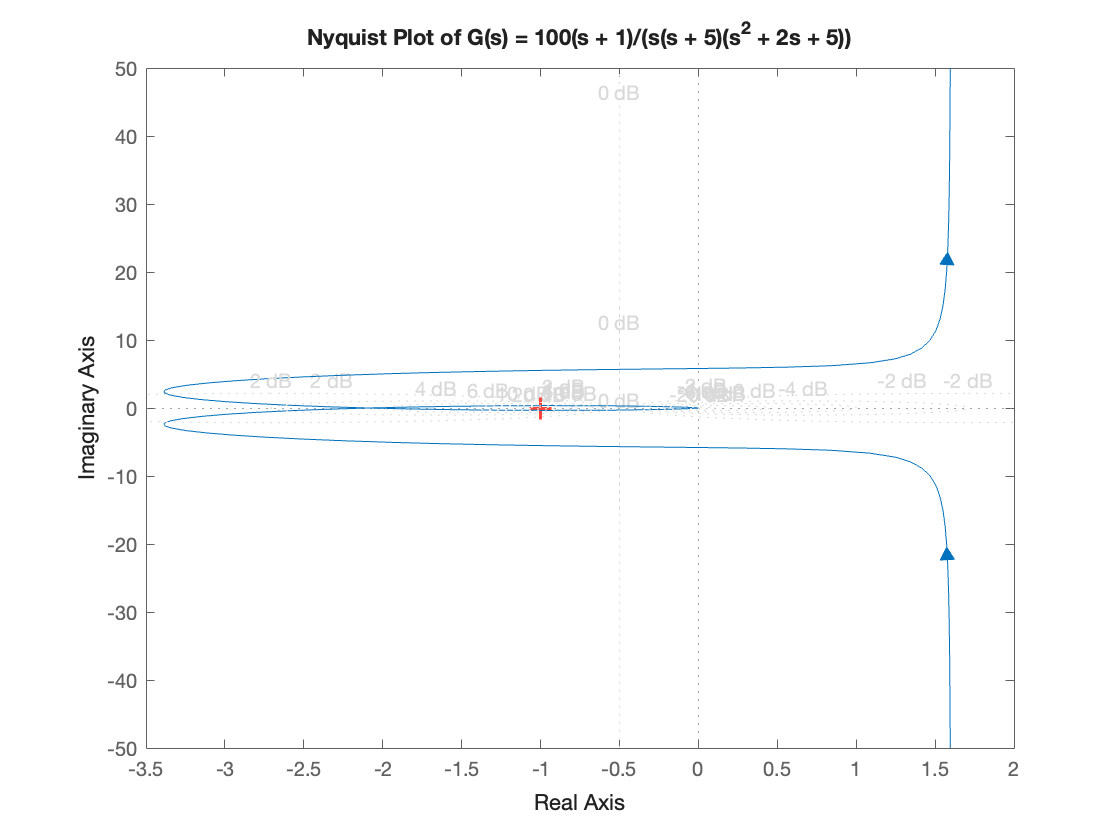
\includegraphics[width=0.9\textwidth]{p2b.png}
    \caption{Nyquist Plot from MATLAB}
    \label{fig:matlab_p3b}
\end{figure}

\begin{resultsbox}
Final answers for the previous problem are summarized in the work above.
\end{resultsbox}

\question{Problem 3 (20 pt)}\label{quest:3}
\begin{stepbox}[Step 1: Approach]
Work through each requested subpart and show supporting derivations.
\end{stepbox}

Consider the linearized modeling of an inverted pendulum on a cart:
\begin{align*}
(M + m) \ddot{x}(t) + b \dot{x}(t) &= f(t) + m l \ddot{\theta}(t), \\
(J + m l^2) \ddot{\theta}(t) - m g l \theta(t) &= m l \ddot{x}(t).
\end{align*}

\begin{enumerate}
    \item[(a)] (10 pt) Let the state variable be \(z = [x, \dot{x}, \theta, \dot{\theta}]^T\). Write the equation of motion in state-space form and identify the \(A\) and \(B\) matrices.

    \item[(b)] (10 pt) Given:
    \[
    M = 1 \, \text{kg}, \quad m = 0.5 \, \text{kg}, \quad b = 0.2 \, \frac{N}{m \cdot s}, \quad l = 0.4 \, \text{m}, \quad J = 0.01 \, \text{kg} \cdot \text{m}^2,
    \]
    use MATLAB to plot the impulse response of the state-space model for 1 second.
\end{enumerate}

\begin{enumerate}
    \item[(a)] \textbf{State-Space Representation}

    The given equations of motion for the inverted pendulum on a cart are:
    \begin{align*}
    (M + m) \ddot{x}(t) + b \dot{x}(t) &= f(t) + m l \ddot{\theta}(t), \\
    (J + m l^2) \ddot{\theta}(t) - m g l \theta(t) &= m l \ddot{x}(t).
    \end{align*}

    Let the state vector be:
    \[
    z = \begin{bmatrix} x \\ \dot{x} \\ \theta \\ \dot{\theta} \end{bmatrix}
    \]

    \textbf{Rewriting the Equations}

    Rearrange the equations to isolate the accelerations:
    \begin{align*}
    (M + m) \ddot{x} - m l \ddot{\theta} + b \dot{x} &= f, \\
    -m l \ddot{x} + (J + m l^2) \ddot{\theta} - m g l \theta &= 0.
    \end{align*}

    Express these equations in matrix form:
    \[
    \begin{bmatrix}
    M + m & -m l \\
    -m l & J + m l^2
    \end{bmatrix}
    \begin{bmatrix}
    \ddot{x} \\
    \ddot{\theta}
    \end{bmatrix}
    =
    \begin{bmatrix}
    f - b \dot{x} \\
    m g l \theta
    \end{bmatrix}.
    \]

    \textbf{Solving for the Accelerations}

    Let:
    \begin{align*}
    a_1 &= J + m l^2, \\
    a_2 &= m l, \\
    a_3 &= M + m, \\
    D &= a_1 a_3 - a_2^2.
    \end{align*}

    Then, the accelerations are:
    \[
    \begin{bmatrix}
    \ddot{x} \\
    \ddot{\theta}
    \end{bmatrix}
    =
    \frac{1}{D}
    \begin{bmatrix}
    a_1 & a_2 \\
    a_2 & a_3
    \end{bmatrix}
    \begin{bmatrix}
    f - b \dot{x} \\
    m g l \theta
    \end{bmatrix}.
    \]

    Expanding, we get:
    \begin{align*}
    \ddot{x} &= \left( -\frac{a_1 b}{D} \right) \dot{x} + \left( \frac{a_2^2 g}{D} \right) \theta + \left( \frac{a_1}{D} \right) f, \\
    \ddot{\theta} &= \left( -\frac{a_2 b}{D} \right) \dot{x} + \left( \frac{a_2 a_3 g}{D} \right) \theta + \left( \frac{a_2}{D} \right) f.
    \end{align*}

    \textbf{State-Space Form}

    The state-space representation is:
    \[
    \dot{z} = A z + B f,
    \]
    where:
    \[
    A =
    \begin{bmatrix}
    0 & 1 & 0 & 0 \\
    0 & -\dfrac{a_1 b}{D} & \dfrac{a_2^2 g}{D} & 0 \\
    0 & 0 & 0 & 1 \\
    0 & -\dfrac{a_2 b}{D} & \dfrac{a_2 a_3 g}{D} & 0
    \end{bmatrix}, \quad
    B =
    \begin{bmatrix}
    0 \\
    \dfrac{a_1}{D} \\
    0 \\
    \dfrac{a_2}{D}
    \end{bmatrix}.
    \]

    \item[(b)] \textbf{MATLAB Code for Impulse Response}

    Given the parameters:
    \[
    M = 1\, \text{kg}, \quad m = 0.5\, \text{kg}, \quad b = 0.2\, \frac{\text{N}\cdot\text{s}}{\text{m}}, \quad l = 0.4\, \text{m}, \quad J = 0.01\, \text{kg}\cdot\text{m}^2.
    \]

    Below is the MATLAB code that calculates the necessary constants and plots the impulse response over 1 second:

    \begin{lstlisting}[language=Matlab]
    % Define the given parameters
    M = 1;        % Mass of the cart (kg)
    m = 0.5;      % Mass of the pendulum (kg)
    b = 0.2;      % Damping coefficient (N/(m*s))
    l = 0.4;      % Length to pendulum center of mass (m)
    J = 0.01;     % Moment of inertia of the pendulum (kg*m^2)
    g = 9.81;     % Acceleration due to gravity (m/s^2)

    % Calculate intermediate constants
    a1 = J + m * l^2;
    a2 = m * l;
    a3 = M + m;
    D = a1 * a3 - a2^2;

    % Calculate elements of the A matrix
    A21 = -(a1 * b) / D;
    A23 = (a2^2 * g) / D;
    A41 = -(a2 * b) / D;
    A43 = (a2 * a3 * g) / D;

    % Calculate elements of the B matrix
    B2 = a1 / D;
    B4 = a2 / D;

    % Assemble the A and B matrices
    A = [0,    1,      0,      0;
         0,   A21,    A23,     0;
         0,    0,      0,      1;
         0,   A41,    A43,     0];

    B = [0;
         B2;
         0;
         B4];

    % Define the output matrix C and direct transmission matrix D_mat
    C = eye(4); % Observing all state variables
    D_mat = zeros(4,1);

    % Create the state-space system
    sys = ss(A, B, C, D_mat);

    % Define the time vector for 1 second
    t = linspace(0, 1, 1000);

    % Plot the impulse response
    figure;
    impulse(sys, t);
    title('Impulse Response of the Inverted Pendulum System');
    xlabel('Time (seconds)');
    ylabel('State Variables');
    legend('x (Position)', 'dx/dt (Velocity)', '\theta (Angle)', 'd\theta/dt (Angular Velocity)');
    grid on;
    \end{lstlisting}

    \textbf{Explanation:}

    \begin{itemize}
        \item \textit{Parameters:} We start by defining all the given physical parameters: $M$, $m$, $b$, $l$, $J$, and $g$.
        \item \textit{Intermediate Constants:} We calculate $a_1$, $a_2$, $a_3$, and $D$ using the given parameters.
        \item \textit{Matrix Elements:} Using the intermediate constants, we compute the individual elements of the $A$ and $B$ matrices.
        \item \textit{State-Space Matrices:} We assemble the $A$ and $B$ matrices using the calculated elements. The output matrix $C$ is set to the identity matrix to observe all state variables. The direct transmission matrix $D_{\text{mat}}$ is a zero matrix since there is no direct feed-through.
        \item \textit{Simulation:} We create a time vector \texttt{t} from 0 to 1 second with 1000 points. We use the \texttt{impulse} function to simulate and plot the impulse response of the system over the specified time.
    \end{itemize}
    \begin{figure}[h!]
    \centering
    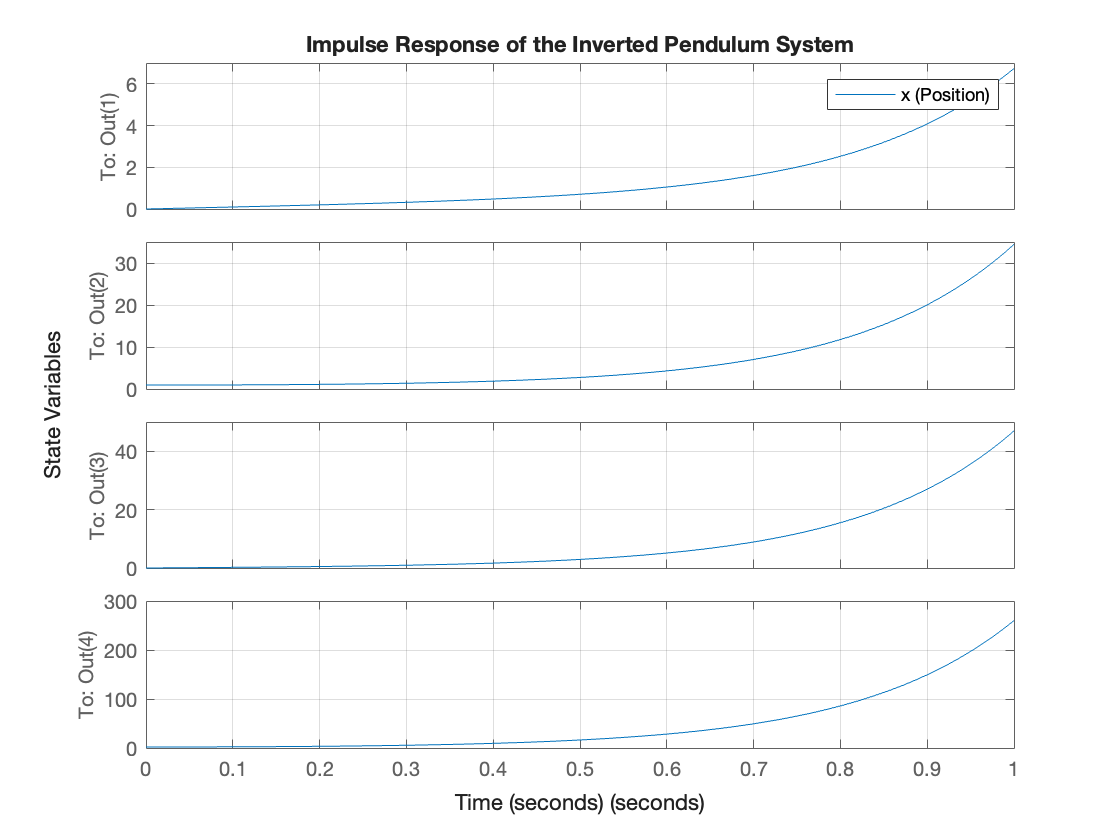
\includegraphics[width=0.9\textwidth]{p3b.png}
    \caption{Plot from MATLAB}
    \label{fig:magnitude}
\end{figure}

\end{enumerate}

\newpage
\begin{resultsbox}
Final answers for the previous problem are summarized in the work above.
\end{resultsbox}

\question{Bonus Problem (20 pt)}\label{quest:4}
\begin{stepbox}[Step 1: Approach]
Work through each requested subpart and show supporting derivations.
\end{stepbox}

Consider the suspension system given in Figure 1. Let the state vector be given by:
\[
z(t) = [x(t), \dot{x}(t), y(t), \dot{y}(t)]^T.
\]
Find the \(A\) and \(B\) matrices of the following state-space equation:
\[
\dot{z}(t) = A z(t) + B u(t).
\]

\begin{center}
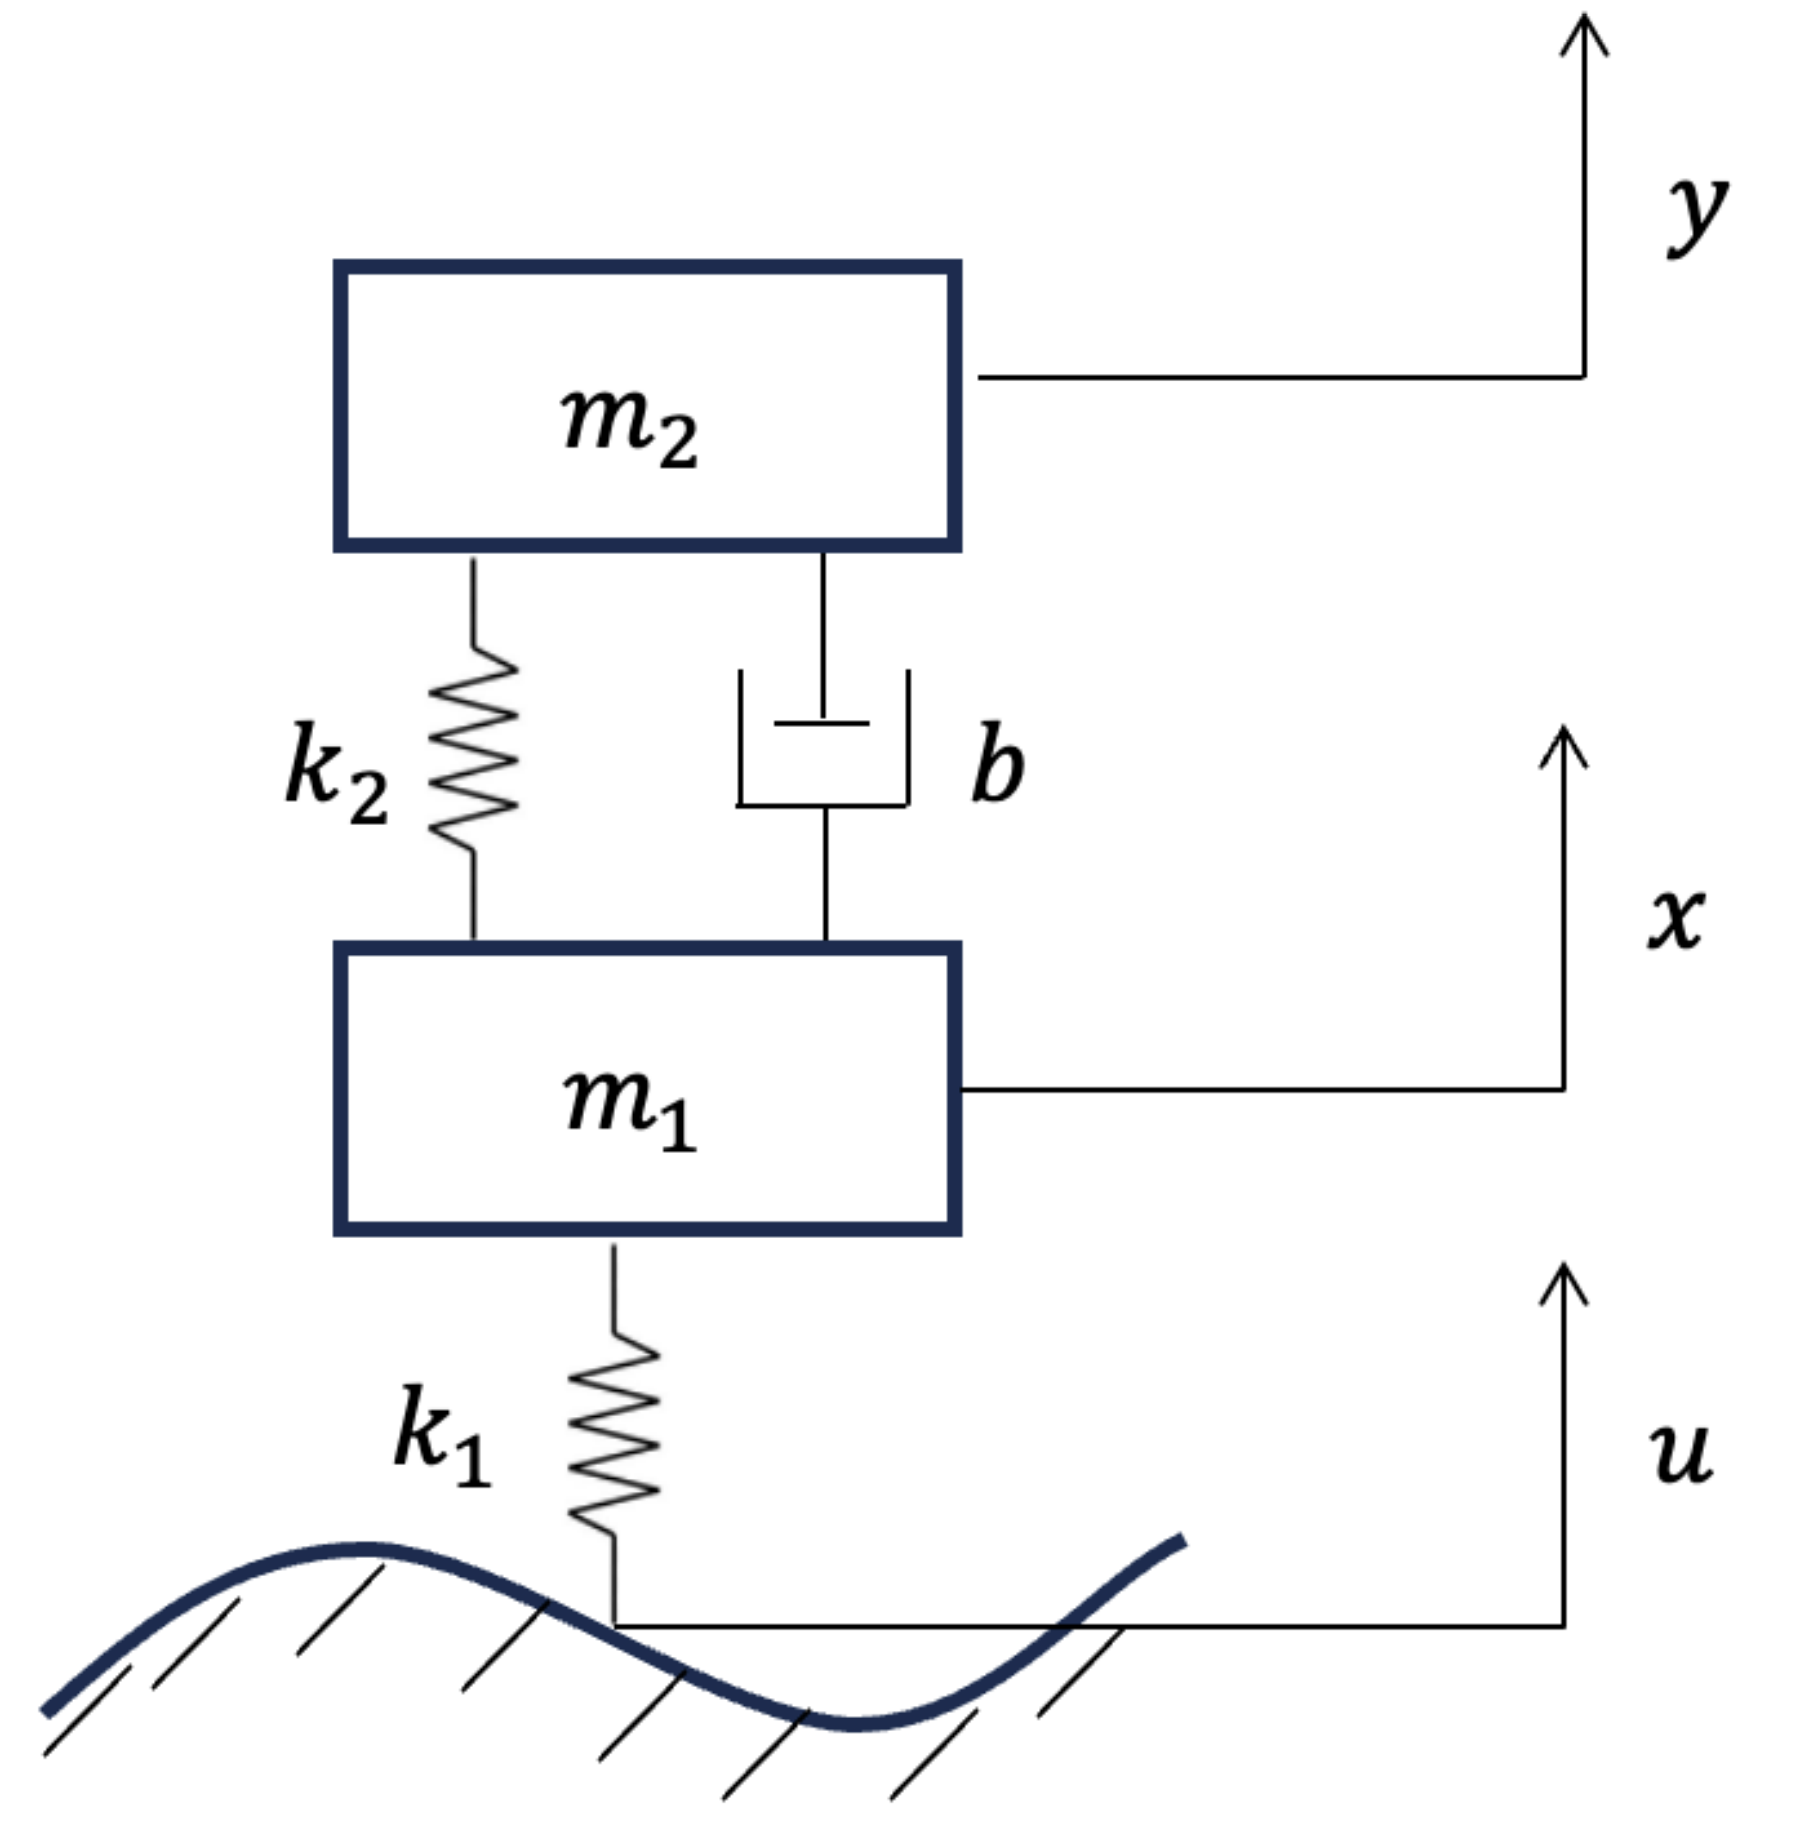
\includegraphics[width=0.5\textwidth]{suspension_system.png}
\end{center}

\subsection*{Understanding the Suspension System}

The suspension system consists of two masses connected by springs and dampers. The movement of these masses is governed by the forces exerted by the springs, dampers, and an external input.

\subsubsection*{Variables and Parameters}

\begin{itemize}
    \item \textbf{Positions:}
    \begin{itemize}
        \item \( x(t) \): Position of Mass 1 at time \( t \).
        \item \( y(t) \): Position of Mass 2 at time \( t \).
    \end{itemize}
    \item \textbf{Velocities:}
    \begin{itemize}
        \item \( \dot{x}(t) \): Velocity of Mass 1.
        \item \( \dot{y}(t) \): Velocity of Mass 2.
    \end{itemize}
    \item \textbf{Accelerations:}
    \begin{itemize}
        \item \( \ddot{x}(t) \): Acceleration of Mass 1.
        \item \( \ddot{y}(t) \): Acceleration of Mass 2.
    \end{itemize}
    \item \textbf{Masses:}
    \begin{itemize}
        \item \( m_1 \): Mass of the first object.
        \item \( m_2 \): Mass of the second object.
    \end{itemize}
    \item \textbf{Spring Constants:}
    \begin{itemize}
        \item \( k_1 \): Spring constant of the first spring.
        \item \( k_2 \): Spring constant of the second spring.
    \end{itemize}
    \item \textbf{Damping Coefficient:}
    \begin{itemize}
        \item \( b \): Damping coefficient representing resistance to motion.
    \end{itemize}
    \item \textbf{External Input:}
    \begin{itemize}
        \item \( u(t) \): External force or displacement acting on Mass 1.
    \end{itemize}
\end{itemize}

\subsection*{Given Equations of Motion}

The dynamics of the system are described by the following equations:

\begin{enumerate}
    \item For Mass 1:
    \[
    m_1 \ddot{x} = k_2 (y - x) + b (\dot{y} - \dot{x}) + k_1 (u - x)
    \]
    \item For Mass 2:
    \[
    m_2 \ddot{y} = k_2 (x - y) + b (\dot{x} - \dot{y})
    \]
\end{enumerate}


\subsection*{Step-by-Step Solution}

\subsubsection*{Step 1: Define the State Variables}

We define the state vector \( z(t) \) as:
\[
z(t) = \begin{bmatrix}
z_1(t) \\
z_2(t) \\
z_3(t) \\
z_4(t)
\end{bmatrix}
=
\begin{bmatrix}
x(t) \\
\dot{x}(t) \\
y(t) \\
\dot{y}(t)
\end{bmatrix}
\]
Thus, our state variables are:
\begin{align*}
z_1(t) &= x(t) \quad \text{(Position of Mass 1)} \\
z_2(t) &= \dot{x}(t) \quad \text{(Velocity of Mass 1)} \\
z_3(t) &= y(t) \quad \text{(Position of Mass 2)} \\
z_4(t) &= \dot{y}(t) \quad \text{(Velocity of Mass 2)}
\end{align*}

\subsubsection*{Step 2: Express Derivatives of State Variables}

The derivatives of the state variables are:
\begin{align*}
\dot{z}_1(t) &= \dot{x}(t) = z_2(t) \\
\dot{z}_2(t) &= \ddot{x}(t) \\
\dot{z}_3(t) &= \dot{y}(t) = z_4(t) \\
\dot{z}_4(t) &= \ddot{y}(t)
\end{align*}

\subsubsection*{Step 3: Rewrite the Equations of Motion Using State Variables}

\paragraph{Equation for \( \dot{z}_2(t) \):}

Starting with the equation for Mass 1:
\[
m_1 \ddot{x} = k_2 (y - x) + b (\dot{y} - \dot{x}) + k_1 (u - x)
\]
Substitute the state variables:
\[
m_1 \dot{z}_2 = k_2 (z_3 - z_1) + b (z_4 - z_2) + k_1 (u - z_1)
\]
Solving for \( \dot{z}_2 \):
\[
\dot{z}_2 = \frac{1}{m_1} \left[ - (k_1 + k_2) z_1 - b z_2 + k_2 z_3 + b z_4 + k_1 u \right]
\]

\paragraph{Equation for \( \dot{z}_4(t) \):}

Starting with the equation for Mass 2:
\[
m_2 \ddot{y} = k_2 (x - y) + b (\dot{x} - \dot{y})
\]
Substitute the state variables:
\[
m_2 \dot{z}_4 = k_2 (z_1 - z_3) + b (z_2 - z_4)
\]
Solving for \( \dot{z}_4 \):
\[
\dot{z}_4 = \frac{1}{m_2} \left[ k_2 z_1 + b z_2 - k_2 z_3 - b z_4 \right]
\]

\subsubsection*{Step 4: Compile All State Equations}

We now have four first-order differential equations:
\begin{align*}
\dot{z}_1 &= z_2 \\
\dot{z}_2 &= \frac{1}{m_1} \left[ - (k_1 + k_2) z_1 - b z_2 + k_2 z_3 + b z_4 + k_1 u \right] \\
\dot{z}_3 &= z_4 \\
\dot{z}_4 &= \frac{1}{m_2} \left[ k_2 z_1 + b z_2 - k_2 z_3 - b z_4 \right]
\end{align*}

\subsubsection*{Step 5: Write in Matrix Form}

We aim to express the system in the state-space form:
\[
\dot{z}(t) = A z(t) + B u(t)
\]
Where:
\begin{itemize}
    \item \( \dot{z}(t) \) is the vector of derivatives of the state variables.
    \item \( A \) is the system matrix representing how the current state affects the rate of change.
    \item \( B \) is the input matrix representing how the external input influences the state.
\end{itemize}

\paragraph{Constructing Matrix \( A \):}

From the state equations, the coefficients of \( z_1, z_2, z_3, z_4 \) form the matrix \( A \):
\[
A = \begin{bmatrix}
0 & 1 & 0 & 0 \\
-\dfrac{k_1 + k_2}{m_1} & -\dfrac{b}{m_1} & \dfrac{k_2}{m_1} & \dfrac{b}{m_1} \\
0 & 0 & 0 & 1 \\
\dfrac{k_2}{m_2} & \dfrac{b}{m_2} & -\dfrac{k_2}{m_2} & -\dfrac{b}{m_2}
\end{bmatrix}
\]

\paragraph{Constructing Vector \( B \):}

Only \( \dot{z}_2 \) is directly influenced by the external input \( u(t) \), so the input matrix \( B \) is:
\[
B = \begin{bmatrix}
0 \\
\dfrac{k_1}{m_1} \\
0 \\
0
\end{bmatrix}
\]

\subsection*{Final State-Space Representation}

Combining the matrices \( A \) and \( B \), the state-space equation is:
\[
\dot{z}(t) = \begin{bmatrix}
0 & 1 & 0 & 0 \\
-\dfrac{k_1 + k_2}{m_1} & -\dfrac{b}{m_1} & \dfrac{k_2}{m_1} & \dfrac{b}{m_1} \\
0 & 0 & 0 & 1 \\
\dfrac{k_2}{m_2} & \dfrac{b}{m_2} & -\dfrac{k_2}{m_2} & -\dfrac{b}{m_2}
\end{bmatrix}
\begin{bmatrix}
z_1 \\
z_2 \\
z_3 \\
z_4
\end{bmatrix}
+
\begin{bmatrix}
0 \\
\dfrac{k_1}{m_1} \\
0 \\
0
\end{bmatrix}
u(t)
\]


\begin{resultsbox}
Final answers for the previous problem are summarized in the work above.
\end{resultsbox}

\end{document}
